%%%%%%%%%%%%%%%%%%%%%%%%%%%%%%%%%%%%%%%%%
% Barbara Liskov Presentation
% LaTeX Template
% 23/11/2020
% 
%%%%%%%%%%%%%%%%%%%%%%%%%%%%%%%%%%%%%%%%%

%----------------------------------------------------------------------------------------
%	PACKAGES AND THEMES
%----------------------------------------------------------------------------------------

\documentclass{beamer}

\mode<presentation> {

\usetheme{Madrid}

}

\usepackage{graphicx} % Allows including images
\usepackage{booktabs} % Allows the use of \toprule, \midrule and \bottomrule in tables

%----------------------------------------------------------------------------------------
%	TITLE PAGE
%----------------------------------------------------------------------------------------

\title[Research Methods]{Barbara Liskov} % The short title appears at the bottom of every slide, the full title is only on the title page
\author{Group N} % Your name
\institute[GMIT] % Your institution as it will appear on the bottom of every slide, may be shorthand to save space
{
\textit{Grace Keane} \\\textit{Shirin Nagle} \\ % Your institution for the title page
\medskip
}
\date{}

\begin{document}

\begin{frame}
\titlepage % Print the title page as the first slide
\end{frame}

%----------------------------------------------------------------------------------------
%	BRIEF DESCRIPTION
%----------------------------------------------------------------------------------------

\begin{frame}
\frametitle{Brief Description} % Table of contents slide, comment this block out to remove it

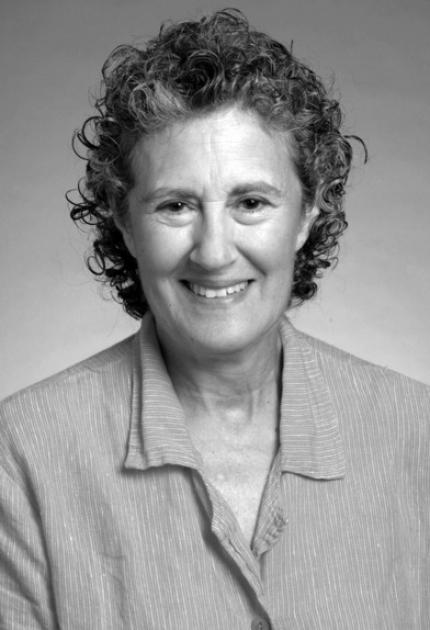
\includegraphics[scale=0.4, align=centre]{Barbara Liskov}
\centering

\end{frame}


%----------------------------------------------------------------------------------------
%	PRESENTATION SLIDES
%----------------------------------------------------------------------------------------

%------------------------------------------------


\begin{frame}
\frametitle{Important Details}
\begin{itemize}
\item Computer Scientist
\item Born: November 7th, 1939, California
\item One of the first women in the USA to be awarded a PhD in Computer Science
\item She is one of the world's leading authorities on computer language and system design
\item She won numerous awards as well as the Turing award
\item Created the Liskov's substitution principle
\end{itemize}
\end{frame}

%------------------------------------------------

\begin{frame}
\frametitle{Contributions}

Barbara Liskov contributed to practical and theoretical foundations of programming language and system design, especially related to data abstraction, fault tolerance, and distributed computing. 

\vspace{5mm} %5mm vertical space
She developed a new notion of sub typing known as the Liskov Substitution principle.


\end{frame}

%------------------------------------------------

\begin{frame}
\frametitle{Turing Award}
\begin{theorem}[Title]
\centering
Liskov Substitution Principle
\end{theorem}
\end{frame}

%------------------------------------------------

\begin{frame}
\frametitle{Title}
\end{frame}

%------------------------------------------------


\begin{frame}
\frametitle{Title}
\end{frame}

%------------------------------------------------

\begin{frame}
\frametitle{Title}
She did not name the Liskov Substitution Principle. Apparently, she received an email in the 90’s by somebody asking her whether he got her principle right, surprising her. She had not known that the principle had borne her name for years in the community.
\end{frame}

%------------------------------------------------

\begin{frame}
\Huge{\centerline{The End}}
\end{frame}

%----------------------------------------------------------------------------------------

\begin{frame}
\Huge{\centerline{Questions?}}
\end{frame}

%-----------------------------------------------
\end{document} 